\documentclass{article}
\usepackage{todonotes}
\usepackage{biblatex}
\usepackage{listings}
\usepackage{color}
\usepackage{copyrightbox}
\usepackage{ccicons}
\definecolor{lightgray}{rgb}{.9,.9,.9}
\definecolor{darkgray}{rgb}{.4,.4,.4}
\definecolor{purple}{rgb}{0.65, 0.12, 0.82}
\lstdefinelanguage{JavaScript}{
  keywords={break, case, catch, continue, debugger, default, delete, do, else, false, finally, for, function, if, in, instanceof, new, null, return, switch, this, throw, true, try, typeof, var, void, while, with},
  morecomment=[l]{//},
  morecomment=[s]{/*}{*/},
  morestring=[b]',
  morestring=[b]",
  ndkeywords={class, export, boolean, throw, implements, import, this},
  keywordstyle=\color{blue}\bfseries,
  ndkeywordstyle=\color{darkgray}\bfseries,
  identifierstyle=\color{black},
  commentstyle=\color{purple}\ttfamily,
  stringstyle=\color{red}\ttfamily,
  sensitive=true
}

\lstset{
   language=JavaScript,
   backgroundcolor=\color{lightgray},
   extendedchars=true,
   basicstyle=\footnotesize\ttfamily,
   showstringspaces=false,
   showspaces=false,
   numbers=left,
   numberstyle=\footnotesize,
   numbersep=9pt,
   tabsize=2,
   breaklines=true,
   showtabs=false,
   captionpos=b
}
\bibliography{bibliography}

\begin{document}

\title{Multiple coordinated views of tree maps on massive geo data}
\author{Robert Schäfer\\ Department of Computer Graphics, Hasso-Plattner-Institut}
\maketitle

\newcommand{\rufu}{Rundfunk \textsc{mitbestimmen}}
\newcommand\hmm[1]{\ifnum\ifhmode\spacefactor\else2000\fi>1000 \uppercase{#1}\else#1\fi}
\newcommand{\cmv}{\hmm{c}oordinated multiple view}
\newcommand{\cmvs}{\hmm{c}oordinated multiple views}

\begin{abstract}
  Visualizing geographical data on a map is both obvious and intuitive.
  Tree maps allow to visualize arbitrary, hiearchical and multidimensional data using nested rectangles.
  While tree maps look similar to a map, the represented information may not be as intuitive and comprehensible.
  There is no predefined layouting for arbitrary data, let alone no well known layouting that everybody feels comfortable with.
  In this thesis, we propose a coordinated multiple view combining the advantages of both.
  The user gets easy access and selects information through a geographical map and that same data will be displayed in a tree map.
\end{abstract}

\section{Introduction}

\subsection{Motivation}


In many cases, insights based on visualization techniques like \cmvs{} are used by experts for strategic decision-making.
Thus, many advanced data visualizations techniques are made exclusively for professionals.

On the other hand, data visualizations widely popular:
Data journalism is one of the emerging fields in journalism.
Facts and figures are the strongest evidence for opinionated journalistic reports.
Not even a football match can do without a number based analysis.

We believe that advanced data visualization techniques can be adopted and used in both an informative and strategic way by professionals as well as lay people.

\subsection{Problem statement}
\todo[inline]{Start off with the problem of tree map vs geo map}

We use data visualizations in the context of the expenditure of public broadcasting fees in Germany.
Since the year 2013 these fees are compulsory for every home in Germany and as a consequence, broadcasting receives €8,000,000,000 annually.
Yet it is subject to little or no public feedback, ranking, or even debate on what constitutes value or quality.
There is neither transparency on how the fees are spent nor a public feedback on how the fees should be spent.

We see a great potential, a win-win situation to be precise, because both payers of the broadcasting fees and broadcasters themselves can benefit from each other.
As of 2013 there is no legal opt-out anymore and people have a strong interest to say how their fees should be spent.
Broadcasters on the other hand can evaluate their program based on the interests delivered by the users.
This reciprocal relationship would create a public feedback for payers and a better program for broadcasters.

This problem is perfectly suitable to be tackled with data visualizations.
\todo[inline]{Explain why data visualization are good for communication}

\subsubsection{Use case specific problems}
There is striking discrepancy of intentions between available metrics and the programme mandate of public broadcasting.
TV ratings are produced by a group of 5000 representative homes equipped with a special TV box, while Radio ratings are carried out by phone surveys over the course of a year.
Although created differently they share the same intention, i.e.\ to sell advertisements.

We suspect that public broadcasting suffers from an overfitting problem:
Since broadcasters have usage data only, they focus too much on people who still listen to the radio and watch TV.
Young people especially show a decreasing interest in conventional mass media which has been shown in surveys.
Public broadcasting fails in that respect that everybody has to pay and thus has a right to get access to information.


\subsection{Aim of the work}
Our goal is to create meaningful data.
This includes to encourage as many people as possible to publish their interests.
It also involves to provide access to information about the preferred broadcasts.
We suggest that users actively publish data and passively examine the summary of data of all users.
Broadcasters on the other side receive the data and evaluate the program and actively change the program according to the interest of the audience.
\todo[inline]{explain feedback loop}
The mentioned data visualization need to be interactive to show the user the desired level of detail.

\subsubsection{Use case specific goals}
We propose the hypothesis that people behave differently when they decide consciously and when they decide with their remote control.
The hypothesis goes even further, explicit interests may fit to the programme mandate of public broadcasting in contrast to TV and radio ratings which are based on usage data.

As the data is usage independent we want to gain knowledge about the entire population including those who don't use broadcasting at all.
In this manner we want to tackle the mentioned overfitting problem.

\subsection{Methodological approach}

We use different visualization techniques on two existing data sets:
\begin{enumerate}
  \item
    A web application called ``Rundfunk MITBESTIMMEN'' with interactive visualizations of user data.
  \item
    A web application with three dimensional visualizations of geographical data provided by the local authorities.
\end{enumerate}


\section{State of the art}
Like every technique, data visualization serves a purpose.
\textcite{Few2013} mentions sense-making (also called data analysis) and communication.
Statistical information is abstract and in data visualization ``we must find a way to give form to that which has none.''\cite{Few2013}



\subsection{Visualization of hierarchical data}
Visualizing hierarchical data has long tradition.
The traditional representation of a tree is a rooted, directed graph with the root node at the top.
An everyday use case is a directory tree example of a file system, e.g. in file browsers or command line utilities like \texttt{tree} in UNIX.
As \textcite{Shneiderman1992} mentions, this visualization becomes increasingly large when displaying more than one node and soon exceeds the entire screen size.
\textcite{Johnson1991} proposes the tree map visualization technique, in which each node is a rectangle whose area is proportional to some attribute, thus making 100\% use of the available screen size.
It is notable that tree maps are structured in the same way like the visualization of a federal state, as seen in figure~\ref{fig:research:treemap}.
The difference is that there is no predefined algorithm for layouting, which brings up one of the major disadvantages of tree maps:
As the algorithm determines the order of placement, small changes in the input data can lead to a large change in the layout of the resulting tree map.
\todo{What are tree maps?}

\begin{figure}[h]
\centering
  \copyrightbox[b]{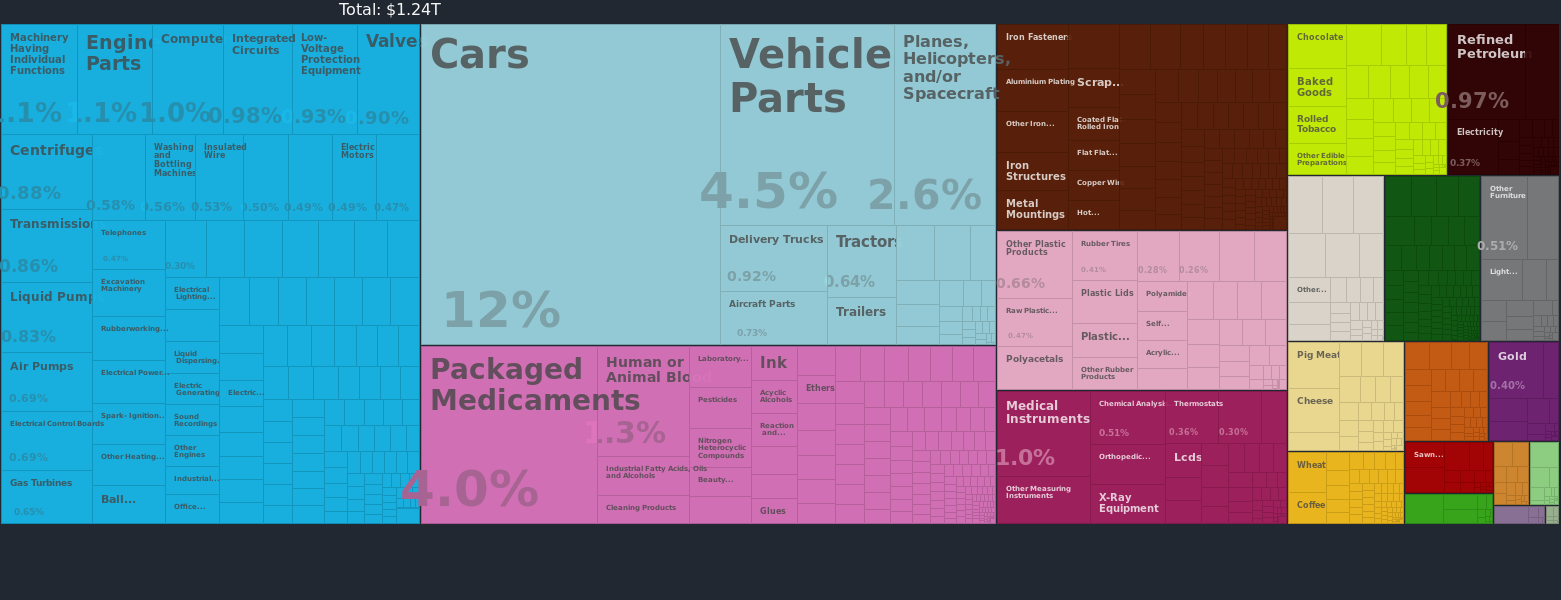
\includegraphics[width=\textwidth]{images/treemap_example}}{ \hfill \ccAttribution \ccShareAlike \hspace{1mm} Observatory of Economic Complexity\cite{Macro2017}}
\caption{German exports visualized as a tree map}
\label{fig:research:treemap}
\end{figure}

In 2004, \textcite{Bladh2004} transfer the concept of tree maps from two dimensional into three dimensional space.
The introduce StepTree, which is a three dimensional tree map to display a directory layout.
It ``differs from Treemap in that it employs three dimensions by stacking each subdirectory on top of its parent directory.''\cite{Bladh2004}
3D tree maps are superior to 2D tree maps for tasks with a pronounced topological challenge.
Yet, 3D visualizations come with other disadvantages as superimposition of objects and a complex view point navigation.
\todo{What are 3D tree maps?}


\todo[inline]{How do tree maps relate to geographical data?}
\subsection{Coordinated multiple views}
According to \textcite{cmv:state_of_the_art} \cmvs{} is just ``a specific exploratory visualization technique that enables users to explore their data''.
\cmvs{} are characterized by the fact, that they show multiple views side-by-side.
Most multiple coordinated views also provide some kind of brushing technique.
``The technique of brushing is the principle approach, where elements are selected (and highlighted) in one display, concurrently the same information in any other linked display is also highlighted.''\cite{cmv:state_of_the_art}
\todo{What are CMVs?}

\begin{figure}[h]
\centering
  \missingfigure{random CMV}
\caption{Example of a \cmvs{}}
\label{fig:research:cmv}
\end{figure}

\section{Methodology}

Since we deal with real world problems, we aim to evaluate the developed tools on real users and existing data.

\subsection{Data sets}
We have two existing data sets:
The first one, called ``RISO'', consists of statistical data from various German administrations.
The second one consists of user data that was collected through a web application called ``Rundfunk MITBESTIMMEN''.

\todo[inline]{Explain the two different data sets}

\subsubsection{RISO}

The RISO data base is used in by local authorities to get insights about governmental KPIs to assist local and regional decision making.
It is a relational database with the three most important tables listed in figure~\ref{fig:data:riso}.
\begin{figure}[h]
\centering
  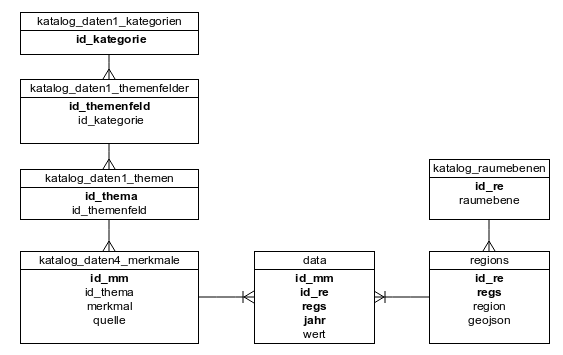
\includegraphics[width=\textwidth]{images/riso}
  \caption{The three most important tables of the RISO database}
  \label{fig:data:riso}
\end{figure}

The largest table is called ``data'', with approximately 10,466,600 records, which holds all values along with the survey date.
This data is connected to a feature table through a foreign key called ``id\_mm''.
In the feature table we can find the description for every referenced feature, e.g. population density, working population in agriculture, education spending.
On the other side, the geometry data is stored in the ``regions'' table and in particular the ``geojson'' column.
The ``data'' and ``regions'' tables are, again, connected via the foreign key ``id\_re''.

The schema of the ``RISO'' database allows to add data of arbitrary size, features and completeness as long as we can store continuous values along withe geometry data.


\subsubsection{Rundfunk MITBESTIMMEN}
Unlike the ``RISO'' database, the schema of ``Rundfunk MITBESTIMMEN'' follows the requirements of a productive web application.
This web application allows user to vote on broadcasts.
Figure~\ref{fig:data:rundfunk} shows how user data is connected to entities, i.e. broadcasts in our use case.
Consequently, the ``users'' table is connected to the ``broadcasts'' table via the ``selections'' table.
The selections table stores the response of a user to the broadcast, e.g. ``positive'' or ``neutral'', as well as an amount in Euro in case the user wants to allocate a share of the monhtly budget to that broadcast.

\begin{figure}[h]
\centering
  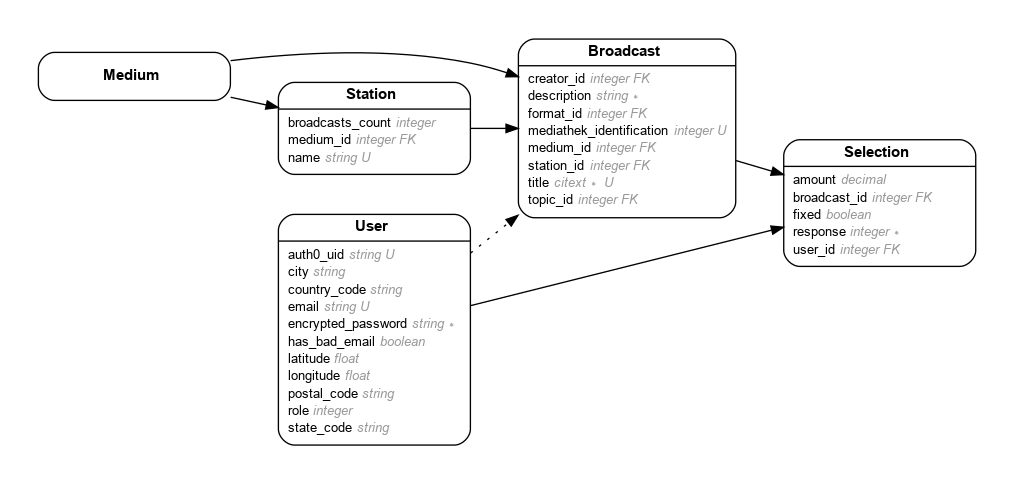
\includegraphics[width=\textwidth]{images/er}
  \caption{Database schema of Rundfunk MITBESTIMMEN app}
  \label{fig:data:rundfunk}
\end{figure}

On both the users table and the broadcast table, we have additional data.
Every user has a \texttt{latitude}, \texttt{longitude} as well as a \texttt{city}, \texttt{postal\_code} and a \texttt{state\_code}.
The broadcast in turn is connected to a \texttt{Station} and also has a \texttt{Medium}.
A station could be a tv or a radio station.
The medium of a broadcast can be one of the following: \texttt{TV}, \texttt{Radio}, \texttt{Online} or \texttt{Other}.
\\
\\
With this data, we can reason about the following questions:
\begin{enumerate}
  \item
    Which broadcasts are selected together very often?
  \item
    Which groups of broadcasts, e.g. all broadcasts of a specific TV station, are performing very well?
  \item
    Wich broadcasts are selected in wich region of Germany?
\end{enumerate}

For the latter, we aggregate the user data with regions and output a geojson file that can be used in our data visualization tool.
Listing~\ref{lst:geojson:example} shows an example.
\lstinputlisting[language=JavaScript, label={lst:geojson:example}, caption={Geojson example}]{listings/example.geojson}


To achieve that we develop a web application where payers of German public broadcasting fees can publish how their broadcasting fees should be spent.
This tool is called \rufu{}.
The workflow goes like this:
\begin{enumerate}
\item Users search for broadcasts
\item Users select broadcasts they want to support
\item Users distribute a virtual budget among the selected broadcasts
\end{enumerate}
\todo[inline]{explain tool in depth}

Considering data visualizations we are facing two challenges in this scenario:
\begin{enumerate}
\item
Visualisations must be easy to understand and intuitive to interact with
\item
Visualizations must be detailed enough to evaluate the program
\end{enumerate}

Make the website user friendly, e.g. guide users as quick as possible to broadcasts they want to support.

\todo[inline]{What did work?}
\todo[inline]{What didn't work?}
\todo[inline]{Current drawbacks}
\todo[inline]{What's missing}




\clearpage
\printbibliography
\end{document}


%Our use case is creating a tool to publicly evaluate public broadcasting in Germany.

%Public broadcasting has a long history in all of Europe.
%Especially after the experiences of the Third Reich, freedom of the press and freedom of broadcasting in particular was defined in the German constitution, the basic law.
%Article 5 not only ensures the press to be free of censorship.
%It is interpreted in such a way that it guarantees broadcasting to exist and be politically and economically independent.
%It is remarkably in many ways:
%First, mass media are recognised to be a basic prerequisite for formation of opinion of the general public.
%Second, the state fosters free access to information, ie. Open Knowledge.

%Despite this highly positive ideal, reality looks somewhat different.
%Public broadcasting in Germany receives €8,000,000,000 (eight billion euros) annually, yet it is subject to little or no public feedback, ranking, or even debate on what constitutes value or quality.
%Since 2013, there is no legal opt-out for German citizen anymore.
%Every home in Germany has to pay for broadcasting whether or not the people actually use it.
%This has created numerous constitutional complaints and approximately 2 million homes in Germany refuse to pay, even it is virtually illegal to do so.

